%%%%%%%%%%%%%%%%%%%%%%%%%%%%%%%%%%%%%%%%%%%%%%%%%%%%%%%%
%
%  FINAL REPORT - Robot Mower
% 
%%%%%%%%%%%%%%%%%%%%%%%%%%%%%%%%%%%%%%%%%%%%%%%%%%%%%%%%
\documentclass[final]{cmpreport_02}


% Some package I am using. You may not need them
%
\usepackage{rotating}
\usepackage{subfloat}
\usepackage{todonotes}
\usepackage{color}
\usepackage{pdfpages}
\usepackage{cleveref}
\usepackage{natbib}
\usepackage{float}
\usepackage{hyperref}
\usepackage{algorithm}
\usepackage{algorithmicx}
\usepackage{algpseudocode}



%\setkeys{Gin}{draft}

%%%%%%%%%%%%%%%%%%%%%%%%%%%%%%%%%%%%%%%%%%%%%%%%%%%%%%%%
%
%  Fill in the fields with:
%
%  your project title
%  your name
%  your registration number
%  your supervisor's name
%
%%%%%%%%%%%%%%%%%%%%%%%%%%%%%%%%%%%%%%%%%%%%%%%%%%%%%%%%
\title{Robot Mower Mapping and Pathing}
%%%%%%%%%%%%%%%%%%%%%%%%%%%%%%%%%%%%%%%%%%%%%%%%%%%%%%%%
%
% The author's name is ignored if the following command 
% is not present in the document
%
% Before submitting a PDF of your final report to the 
% project database you may comment out the command
% if you are worried about lack of anonimity.
%
%%%%%%%%%%%%%%%%%%%%%%%%%%%%%%%%%%%%%%%%%%%%%%%%%%%%%%%%
\author{Toby William Towler}

\registration{100395626}
\supervisor{Edwin Ren}

%%%%%%%%%%%%%%%%%%%%%%%%%%%%%%%%%%%%%%%%%%%%%%%%%%%%%%%%
%
% Fill in the field with your module code.
% this should be:
%
% for BIS project module   -> CMP-6012Y
% for CS project module    -> CMP-6013Y
% for MComp project module -> CMP-7043Y
%
%%%%%%%%%%%%%%%%%%%%%%%%%%%%%%%%%%%%%%%%%%%%%%%%%%%%%%%%
\ccode{CMP-6013Y}

%%%%%%%%%%%%%%%%%%%%%%%%%%%%%%%%%%%%%%%%%%%%%%%%%%%%%%%%
%
% Comment out if confidential report.
% The command should be used if the project is subjected 
% to a Non Disclosure Agreement.
%
% Three examples of the use of the \confidential command. 
% Please ask your supervisor what confidential statement 
% should be used, if appropriate.
%
%%%%%%%%%%%%%%%%%%%%%%%%%%%%%%%%%%%%%%%%%%%%%%%%%%%%%%%%
%\confidential{}

%\confidential{The contents of this report remain confidential for two years and should not be discussed or disclosed to any third party without the prior written permission from the School of Computing Sciences, the University of East Anglia}

%\confidential{The information contained in this document is confidential, privileged and only for the information of the intended recipient and may not be used, published or redistributed without the prior written consent of FruitName Ltd}

\summary{
The abstract of your report summarises your entire work () in no more than half a page. It should include the context of your work including its main objective, what methods you employed, how you implemented these, what the outcomes were and a final statement as a conclusion. It should not contain acronyms, abbreviations, elements of a literature review (though a statement of related work is permissible if it is crucial to your work) or future work. The abstract should be written when everything else has been written up and the project is finished! is this workng
}

\acknowledgements{
    Edwin Ren, Eden Attlebourgh
}

%%%%%%%%%%%%%%%%%%%%%%%%%%%%%%%%%%%%%%%%%%%%%%%%%%%%%%%%%%%%%%%%%%
%
% If you do want a list of figures and a list of tables
% to appear after the table of contents then comment this line.
% THIS IS NOT ADVISED THOUGH AS IT COUNTS FOR YOUR 40 PAGES!
%
% Note that the class file contains code to avoid
% producing an empty list section (e.g list of figures) if the 
% list is empty (i.e. no figure in document).
%
% The command also prevents inserting a list of figures or tables 
% anywhere else in the document
%
%%%%%%%%%%%%%%%%%%%%%%%%%%%%%%%%%%%%%%%%%%%%%%%%%%%%%%%%%%%%%%%%%%
%\nolist

%%%%%%%%%%%%%%%%%%%%%%%%%%%%%%%%%%%%%%%%%%%%%%%%%%%%%%%%%%%%%%%%%%
%
% Comment out if you want your list of figures and list of
% tables on one page instead of two or more pages, in particular 
% if the lists do not fit on a single page.
%
%%%%%%%%%%%%%%%%%%%%%%%%%%%%%%%%%%%%%%%%%%%%%%%%%%%%%%%%%%%%%%%%%%
% \onePageLists


\begin{document}

\section{Introduction}

The robot mower is an already existing project developed by previous masters students from the University of East Anglia.
Physically, the mower has 2 tracks for movement on the sides of a metal frame, it is controlled by raspberry pi 4 running the Robot Operating System \citep{doi:10.1126/scirobotics.abm6074}.
Sensor wise, the robot is equipped with a 4G dongle, lidar and a GPS chip that was upgraded to an RTK chip in this iteration of the project.
The existing code base was mostly written in python with very small amounts of C++.
Because of this, all of my code will be written in python to slot into existing code without issue.

My contribution to this project this year will be, regarding the overall movement and guidance of the robot.
For ease of planning, I have broken this down into 3 sections:
\begin{enumerate}
	\item Basic map generation
	\item complete coverage path planning
	\item map generation from an aerial image
\end{enumerate}

These sections are all modular meaning they can be developed, tested and function independently but still easily be integrated together for the final product.
The specified use case of the robot will now be to cut golf courses, this is particularly relevant to the aerial map generation section of my work which will likely use a machine learning model and require relevant training data, while the other sections are not concerned with a real world use case as their algorithms will work be able to tweaked for any applicable use case of this robot.





\section{Background and Related Work}

Another section that is essential and should keep its title as is! Although you could perhaps call it ``Literature Review'' instead, this is not advisable as at this stage of your project we do not expect an extensive literature review since this was already done in the second formative assignment. The rationale is simply because you will lose valuable pages that could be used better in the next two sections that will cover the preparation and implementation of actual work done. So just provide the context in which your project operates here, and then provide a brief overview of similar work that is directly relevant to yours. Try to avoid blatant copying and pasting from the formative literature review as it is bound to read awkwardly.

\section{System Design}

\subsection{Map Generation}
Map generation is an important part of testing this system, it is important to test on all scenarios that may occur in the real world.
For this reason, random or parameter based map generation is very necessary to guarantee success in every environment.
As the outputs of this section will mostly be used for testing the path planning algorithm on regions with differing area, number of corners and complexity, no excessive algorithmic complexity is needed.
This program should also be able to create n obstacles within the main field, such areas would represent obstructions in the mowers desired path, for example trees or telephone poles in the real world.
This means we need a function with 2 parameters:

\begin{itemize}
	\item \textbf{K}, number of angles in the outer field
	\item \textbf{N}, number of obstacles within the field, since it would not be sensible to take a parameter for the number of corners for every hole, we can generate them randomly assuming 3–8 corners staying inline with the complexity of the rest of the field without being unreasonably overengineered.
\end{itemize}


\subsubsection{Corners}
The number and distance between corners could be thought to represent complexity of a shape.
The number of corners in a shape

KEEPGOING

\subsubsection{Obstacles}
Obstacles or holes, can be thought to represent real world obstructions for example trees or telephone poles in a real field.
Generation of obstacles can be completed using the same function as the outer field generation, simply with different parameters.
The algorithm \ref{mg:genPoints} takes 3 parameters, number of points in the shape, an origin point and the range new points.
This allows for variable size, positioning and complexity.


\subsubsection{Graham Scan}
The Graham Scan \citep{graham1972efficient} is an algorithm to find convex hulls, that is from a set of points the outline which contains all inner points.
This algorithm does this by sorting the points by their polar angle to the lowest point, since this is always in the hull.
There is then further calculations based on the angle between adjacent points to omit inner points from the outline, however for this use case that is not necessary since all points will be vertexes in a field.
For this reason, the algorithm used is not strictly a Graham Scan but rather heavily based on the first stage, as shown in \ref{mg:sortPoints}
Using this algorithm allows for consistent outlining of any set of points with no crossovers or intersections

\subsection{Complete Coverage Path Planning}
Complete coverage path planning(CCPP) is "the task of determining a path that passes over all points of an area or volume of interest while avoiding obstacles" \citep{zhao2023complete}
For this module, I have used the Fields2Cover library \citep{fields2cover}, this library is open source.
During the course of this project, I contributed to his library, fixing a bug during the build process.
The library splits the task up into several sub-tasks.


\subsubsection{Robot Configuration}
Robot sizing has 2 important factors, track width, how wide the machine itself is, and blade width, how wide the utility object is.
For farming equipment the utility object is usually larger than the vehicle, for example a combine harvester's wheels being narrower than blade, however for this project the blade is within the tracks.
For this reason the functions will compute slightly differently to its probable intended use case as the tracks are likely to overlap however this should not cause an issue and all outputs should function as needed.

The robot has 2 more parameters regarding its turning circle, these are minimum turning radius and maximum differential curvature.
Both of these are important when calculating a path for the robot to follow as they ensure the robot can easily follow the path.

The robot is 22cm wide from outer edge to edge and the gap between the tracks is 17cm, with a track width of roughly 2.5cm.


\subsubsection{Headland Generation}
Headlands are the area in which a vehicle turns, think of the rough edges of a crop field, these exist so that agricultural vehicles do not trample their crops when turning.
Although for the use case of a golf course this is not strictly needed as there are no "crops" or areas the robot cannot touch
Headlands are also generated around obstacles to allow for suitable turning area around the obstacles if needed, this serves as an area to do a "U-turn", effectively the same as reaching the end of the field.

KEEPGOING



\subsubsection{Swath Generation}
Swaths are the individual straight lines that make up the complete path,
they are often parallel to each other, but this can vary depending on how the shape of the field is segmented into smaller shapes however they will always be parallel while in the same sub area.
There are 2 ways of determining the optimal angle; the sum of the lengths of all swaths, or the number of swaths, where lower is better for each.
Both of these have pros and cons, for example lower total length offers better time efficiency assuming a near constant travel speed while lower swath count gives reduced turning movements which can be better if turning requires a slower speed or other complexities.
Similarly, lower sum length of course means less distance travelled and usually less fuel/energy consumed, however the opposite can be true if the acceleration and deceleration causes greater energy consumption compared to constant velocity.
Swaths are generated within the bounds of the headlands to allow for independent handling of the turning and connection of swaths regardless of the rest of the generation process.
To find the best angle, each angle is tested and compared. This brute force approach could be considered slow, but it is all the library offers and could be taken into consideration in a future release.

\subsubsection{Route Planning}
A route is the order in which swaths will be covered.
These can be sorted in a number of ways:

\begin{itemize}
	% \item{\textbf{Shortest route} to cover all swaths, ojkrder depends on field}
	\item{\textbf{{Boustrophedon order}, a zigzag like pattern covering swaths in order (1,2,3...)}
	\item{\textbf{Snake order}, Similar to Boustrophedon but skipping 1 swath each time (1,3,5...)}
    \item{\textbf{Spiral order}, a spiral pattern around the field, first swath then last (1, n, 2, n-1...)}
	\item{\textbf{Custom order}, user defined}
\end{itemize}
While they all ensure complete coverage, each of these has their benefits:

Boustrophedon is the most efficient for rectangular shapes, minimising the number of turns and therefore wasted time and energy.

Snake order is the same as boustrophedon but provides a better solution when turning radius is large or multiple passes are needed to completely cover the area.

\todo{turing circle etc}


Spiral order can be benificial in irregular or circular areas where back and forth patterns cause a large number of unnecessary turns.
It also prevents going back over already covered areas which provides greater time efficiency.

Since all of these have their specific use cases it would not make sense to pick one for all appliactions, instead it should be considered for each generation by the user.

\subsubsection{Path Planning}
Path planning refers to the connection of all swaths in route order.
There are a couple of ways the to link neighbouring swaths, these are the Dubins curve and Reeds-Shepp curve.

% \begin{itemize}
% 	\item{Dubins Curve}
% 	\item{Reeds-Shepp curve}
% \end{itemize}

Both of these compute the shortest path between the 2 points, with the deciding factor between the 2 is the robots ability to move backwards.
Reeds-Shepp allows backwards movement


\subsubsection{Cell Decomposition}






\subsection{Aerial Map Generation}
Previously, for the program to take in a real world map from an image of the real world, the user would have to upload the picture and manually trace the outline, this could cause some problems.
For example, the outline is only as accurate as the user's mouse placement, likely skipping some smaller corners to save time or due to inability to be accurate to the necessary degree.
Automating this labourious and time consuming task would positively increase user experience and usability, this can be done using algorithmic and machine learning approaches.

\subsubsection{Algorithmic Approaches}
There are several algorithmic methods that try to achieve this task from several different librarys. A popular library for image processing is scikit-image.

OpenCV's Canny edge detection implementation \citep{opencv_library} follows the classic algorithm developed by Canny \citep{canny1986computational}.
The algorithm works through several steps to detect edges in images:
\begin{itemize}
	\item \textbf{Gaussian Blur}: First, the image is smoothed with a Gaussian filter to reduce noise, as edge detection is highly sensitive to noise.
	\item \textbf{Gradient Calculation}: The algorithm calculates the intensity gradients of the image using Sobel filters in both horizontal and vertical directions:
	\item \textbf{Non-maximum Suppression}: This step thins out the edges by keeping only the local maxima. For each pixel, it checks if it's a local maximum in the direction of the gradient. If not, it's suppressed (set to zero).
	\item \textbf{Double Thresholding}: The algorithm applies two thresholds:
	      \begin{itemize}
		      \item High threshold: Pixels above this are considered "strong" edges
		      \item Low threshold: Pixels between low and high are considered "weak" edges
	      \end{itemize}
	\item Edge Tracking by Hysteresis: Finally, weak edges that are connected to strong edges are kept, while isolated weak edges are discarded. This helps ensure that the detected edges are continuous.
\end{itemize}
This approach works very well for high contrast images, particularly those black and white~\Cref{am:cannyexample}. The clear separation between foreground and background elements allows the algorithm to detect distinct gradient changes and create clean, continuous edge lines.

As for the similarly coloured golf course images, it can often find the outlines but they are made up of many smaller lines~\Cref{am:CannyGolfCourse}. This fragmentation occurs because the subtle color transitions between different areas of the golf course (like fairways, roughs, and greens) create weaker gradient signals that may fall inconsistently above or below the detection thresholds.

It may appear there is a simple solution to this problem; join the connected lines into one, however this proves to be rather problematic in itself for a number of reasons:

\begin{enumerate}
	\item The desired line does not form a complete shape - Gaps in the detected edges mean that even sophisticated line-joining algorithms may fail to connect all segments belonging to a single boundary

	\item The line is connected to other lines outside the desired shape - Many detected edges from shadows, texture variations, or other regions of the golf course can intersect with the boundary edges required to be isolated, creating unwanted connection points

	\item Once lines are connected, it is impossible to tell which collection of lines is needed - Without prior knowledge of the expected shape or additional contextual information, there's no reliable way to determine which edge segments represent meaningful boundaries, like the edge of a green compared to an outline of trees or a rough area.
\end{enumerate}
All of these means use of canny edge detection can often cause more problems than it solves, while it may have more accurate outlines in places, they may be connected to unwanted areas, Or they may not be complete and still require further user input to chose a selection or finish a shape.

\subsubsection{Machine Learning Approach}
Another possible solution to this problem is to use a machine learning network to predict the areas of the golf course instead.
PyTorch \citep{paszke2019pytorch} is a powerful open-source machine learning library and has become one of the most popular frameworks for deep learning research and production applications since its initial release in 2016.
It was developed to show that usability and speed can both be present in a python implementation of machine learning making it the perfect tool for this task.

\subsubsection{Data Set}
A models training data needs to be closely related to its real world input data, for the Robot Mower that is satelite images or orthophotos from above the desired mowing area.
Training data also needs to be clearly and consistently annotated to producde accurate, reliable results in practice.
The only orthophoto data set publicly available is the danish golf course data set, but it lacks quality and consistency; the outlines do not cover the whole area of single sections and often are missing entirely.
Upon testing the data, it produced faulty results including both true negative and false positives. ~\Crefrange{am:AGDanish}{am:ohGCDanish}

A custom data set was needed, or at least custom annotations of the plain images from the Danish data set since the raw images from the data set are still good quality, high resolution images and are suitable for training purposes with correct annotations
\subsubsection{Training}
Pytorch has several training parameters each with their own effect on the outcome. Some foundational hyperparameters are:

\begin{itemize}
	\item{\textbf{Batch size}, determines how many samples are at once, this is mainly limited by available memory}
	\item{\textbf{Image size}, the dimensions of the image, impacting detail perception and processing requirements}
	\item{\textbf{In channels}, depth of input data(RGB vs grayscale)}
	\item{\textbf{Learning rate}, how fast weights are updated during training}
	\item{\textbf{Number of classes}, the amount of classes the model can pick from}
\end{itemize}
There are a few other options needed in the configuration of the model:

% Batch size determines how many samples are processed simultaneously, directly affecting training speed and memory consumption. Image size refers to the height and width dimensions of input images, which impacts model detail perception and computational requirements. In channels represent the depth of input data (3 for RGB images, 1 for grayscale), defining the initial layer's input dimensions. The learning rate controls how quickly model weights are updated during training, with higher values enabling faster learning but potentially overshooting optimal solutions. Finally, the number of classes specifies the output dimension for classification tasks, determining how many different categories the model can predict.

% Foundational hyperparameters include batch size $\text{BATCH\_SIZE} = 4$, input resolution $\text{IMAGE\_SIZE} = (256, 256)$, RGB channels $\text{IN\_CHANNELS} = 3$, learning rate $\text{LEARNING\_RATE} = 1 \times 10^{-3}$, and number of segmentation classes $\text{NUM\_CLASSES} = 6$. To address class imbalance, each class receives a distinct weight $\text{CLASS\_WEIGHTS} = [0.5, 1.0, 2.0, 2.5, 2.0, 1.5]$, with higher weights assigned to less frequent classes.

\textbf{Class weights} are distinctly assigned to each class, higher weights are given to less frequent classes to help balance the less frequent outputs.

Data augmentation enhances the model's robustness with random horizontal and vertical flips (probability $P = 0.5$ for each), random rotations $\theta \sim \mathcal{U}(-20^{\circ}, 20^{\circ})$ with $P = 0.5$, color jitter transformations for brightness, contrast, and saturation $\sim \mathcal{U}(0.8, 1.2)$ with $P = 0.5$, and random crops to 80\% of original size with $P = 0.5$.

The network architecture follows an enhanced UNet design with an encoder channel progression $[3 \rightarrow 24 \rightarrow 48 \rightarrow 96]$, bottleneck channels $192$, and symmetric decoder. Memory efficiency is achieved through depthwise separable convolutions (kernel size $3 \times 3$, padding $1$, groups equal to input channels) and squeeze-excitation blocks with reduction ratio $4$.

For optimization, the model employs a combined loss function $\mathcal{L}_{\text{total}} = 0.7 \cdot \mathcal{L}_{\text{CE}} + 0.3 \cdot \mathcal{L}_{\text{Dice}}$, where $\mathcal{L}_{\text{Dice}} = 1 - \frac{2 \cdot \text{intersection} + 1.0}{\text{union} + 1.0}$. Training utilizes the AdamW optimizer with learning rate $\eta = 1 \times 10^{-3}$ and weight decay $\lambda = 1 \times 10^{-4}$. A OneCycleLR scheduler manages learning rate progression with parameters $\text{pct\_start} = 0.1$, $\text{div\_factor} = 10$, $\text{final\_div\_factor} = 100$, and $\text{three\_phase} = \text{True}$.

The PyTorch Lightning trainer configuration includes $\text{max\_epochs} = 100$, mixed precision training ($\text{precision} = \text{``16-mixed''}$), gradient clipping ($\text{gradient\_clip\_val} = 0.5$), gradient accumulation ($\text{accumulate\_grad\_batches} = 2$), and validation metrics checked every quarter epoch ($\text{val\_check\_interval} = 0.25$) using half the validation data ($\text{limit\_val\_batches} = 0.5$). Early stopping monitors validation IoU with patience of 15 epochs, while the model checkpoint system saves the top 2 models based on validation performance.

Dataset partitioning allocates 70\% for training, 20\% for validation, and 10\% for testing. Full-resolution inference processes images in patches of size 256 with 50\% overlap, employing test-time augmentation by averaging predictions from the original image and its horizontal and vertical flips for improved robustness.

\todo{Random forest or not?}
To ensure consistent training and results, the data set is split up into sections; 70\% for training, 20\% for validation and 10\% for testing.
Constant validation helps to make sure that the model is constantly improving, tweaking the hyperparameters and make modelling decisions.
\section{Performance Evaluation}
Performance is a key part of user experience therefore is crucial to the real world performance of this product.
Performance in this case can be broken down into 2 key metrics:

\begin{itemize}
    \item{\textbf{Run time}: how long the process takes to complete in real time}
    \item{\textbf{Memory Usage}: how much system memory the process uses both average and maximum}
\end{itemize}

Both of these can be measured in python consistently and reliably, meaning the code can be directly tested in the same file without needing system usage or other programs that may have their own overheads.
Each module will be run with different parameters to see how they impact performance which then will be run 5 times,
these 5 results will then be averaged and plotted against the chosen parameter providing clear graphs to visualise any impact varying inputs may have on the products performance.
A baseline run will be provided using set parameters and run 10 times to show a good default.

Run time will be measured in milleseconds and track the total execution time from start to finish. 
The tool used to measure exectuion time  is the \textbf{time} library and its \textbf{perf\_counter} function.
This is accurate to nanoseconds and causes negligable difference in runtime.

Memory Usage will be measured in MB and track the average and peak memory usage during the runtime of the program.
Peak memory usage is tracked using the \textbf{tracemalloc} library.
This library tracks the peak memory usage of the code exectuion.

For reference, these benchmarks were taken on a \textbf{Ryzen5 5600X} with \textbf{16GB} of R.A.M. at \textbf{3200 MT/s}.

\subsection{Map Generation}
\subsubsection{Run Time}
\paragraph{BaseLine} \

\Cref{PE:mg:baselineRT} represents the baseline and tested with 10 corner points, 0-400 range and 0 holes.
The runtime is fairly consistent having a very small range of 0.2 milleseconds, showing a very strong baseline to run further testing on.


\paragraph{Number of points} \

\Cref{PE:mg:points} shows the impact of varying the number of points on runtime.
The tests were run with a range or 0-400 and 0 holes.
Clearly points are added in linear respect to execution time but are efficient in doing so, taking around 0.0075 milleseconds per point added.
Points are added with O(n) complexity


\paragraph{Range of points} \

\Cref{PE:mg:range} visualises the time taken when varying limits are placed on the range of points, this can be thought to represent the Physical size of the field.
These runs were carried out with 10 points and 0 holes.
There is no clear correlation between the range of points and the run time of the program, the graph closely resembles the baseline, having the same range and very similar bounds at each side.
The quickest runtime from this test and all baseline runs actually occurs with a range 1200, three times the range in the baseline.
This is a very good indication on top of everything else that range has no effect on runtime meaing the program should work for any size of field in good time.

\paragraph{Number of holes} \

\Cref{PE:mg:holes} demonstrates how the number of holes translate to runtime.
The runs were carried out with 10 points in the main field, a range of 400 and 5 points in each hole.
Similarly to the number of points, the number of holes has a linear effect on runtime, however runtime increaes in larger steps.
This is likely because in this example, each hole has 5 points and an extra append operation, this is likely why the same number of points generated in the outside field, and in total considering holes differ in runtime.
For instance, 200 points in a single field takes around 1.5ms but 210 points comprised of 10 in the outer field and 40, 5 point holes just under 2ms.
This time increase does not line up and could be for a number of reasons such as the additional appending to the array or the random number generation process of the point generation function, or could be the extra overheads from the sorting of the points in each hole.
Whichever of these is the cause, or if it is a combination of all 3, they are all needed operations so nothing can be done to improve this further, although they whole process still completes in an insignificant amount of time, even with 200 holes it only takes around 9 milleseconds.
200 holes is likely far more than any real world appliaction would need but still computes in excellent time.


\subsubsection{Memory Usage}

\paragraph{Baseline} \

\Cref{PE:mg:memBaseline} is a baseline graph to show the memory usage of the map generation process with 10 points, 400 range and 0 holes.
There memory usage is quite consisten except for the obvious outlier on run 1.
There is no clear reason for this but it occured on every measurement taken, it is possible it is an issue with the measurement script although unlikely.


\paragraph{Number of points} \

\Cref{PE:mg:memPoints} shows the memory usage of the map generation process with variable points, 400 range and 0 holes.
Points effect memory linearly which make sense as there is contasnt size need for each point.
The amount of memory needed is very small and is almost guaranteed to be suitable for any computer system even a low end portable micro PC such as a raspberry Pi.


\paragraph{Range of points} \

\Cref{PE:mg:memRange} draws the memory usage of the map generation process with 10 points, variable range and 0 holes.
Increasing the range of points does have a positively correlated effect on memory when compared to the baseline.
This could be for a number of reasons but essentially comes down to the higher number possible coordinate values.
That could be the data structure of the point takes more memory to store the greater value, because the random number generation process requires more memory or becuase the sorting algorithm needs to memory to sort the higher values.

\paragraph{Number of holes} \

\Cref{PE:mg:memHoles} demonstrates the memory usage of the map generation process with 10 points, 400 range and variable holes.
As mentioned in the runtime section, holes are closely related to points, they effect memory linearly, but at a higher rate than points as they are a collection of points.
Where memory differs to runtime however, is there are no overheads to having points as holes or a single field, since memory allocation is constant.
This concludes the number of holes is irrelevant and the number of total points is all that needs to be considered.


\subsection{Complete Coverage Path Planning}
\subsubsection{Runtime}
\paragraph{Basaeline} \

\Cref{PE:p:baseline} shows a baseline runtime for the fields2cover library generating with:

\begin{itemize}
    \item{\textbf{Area}, 10^5m^2 and 6 sides}
    \item{\textbf{Mower size}, 0.22m track wide, 0.15m working width}
    \item{\textbf{Headland generation}, constant function}
    \item{\textbf{Swath generation}, brute force}
    \item{\textbf{Route planning}, boustrophedon order}
    \item{\textbf{Path planning}, dubins curve}
    \item{\textbf{Cell decomposition}, none}
\end{itemize}
These paremters are all default, the first mentioned or most simplistic to give a stable baseline.

\paragraph{Map Size} \

\Cref{PE:p:setSize} shows how differing field size affects the runtime of algorithm.



y axis - memory usage
x axis - map size

y axis - run time
x axis - map size

y axis - memory usage
x axis - route planning method

y axis - run time
x axis - route planning method

y axis - memory usage
x axis - map shape (cornes, sqaure vs star shape etc)

y axis - run time
x axis - map shape

\subsection{Aerail Map Generation}

y axis - accuracy
x axis - image size

y axis - accuracy
x axis - image resolution

y axis - accuracy
x axis - training data size

y axis - accuracy
x axis - training epochs

y axis - precision
x axis - recall
\section{Conclusion and Future Work}


Another essential section that should keep its title as suggested. Briefly discuss your main findings, outcomes, results; what worked and what could have been done differently. Then summarise your work in a concluding statement by comparing your outcomes against the main and sub-objectives and/or MoSCoW requirements (if used) and suggest potential future work that could be done if more time would be available.


\clearpage

\bibliography{reportbib}

\appendix
\clearpage

\section{Map Generation}

\begin{algorithm}[h!]
	\caption{Point Class Definition}
	\label{mg:point class}
	\begin{algorithmic}[1]
		\Procedure{class Point}{}
		\State $X \gets -1$ \Comment{X-coordinate initialized to -1}
		\State $Y \gets -1$ \Comment{Y-coordinate initialized to -1}
		\State $angle \gets -10$ \Comment{Angle initialized to -10}
		\Procedure{Constructor}{$x$, $y$}
		\State $this.X \gets x$
		\State $this.Y \gets y$
		\State $this.angle \gets -10$ \Comment{Default angle value}
		\EndProcedure
		\EndProcedure
	\end{algorithmic}
\end{algorithm}

\begin{algorithm}[h!]
	\caption{Generate random points}
	\label{mg:genPoints}
	\begin{algorithmic}[1]
		\Function{GenPoints}{$num$, $P$, $size$}
		\State $points \gets []$
		\For{$i \gets 0$ \textbf{to} $num - 1$}
		\State $randX \gets \text{random\_integer}(P.X + 1, P.X + size)$
		\State $randY \gets \text{random\_integer}(P.Y + 1, P.Y + size)$
		\State $points.\text{append}(\text{Point}(randX, randY))$
		\EndFor
		\State \Return $points$
		\EndFunction
	\end{algorithmic}
\end{algorithm}

\begin{algorithm}[h!]
	\caption{Sort points by polar angle to origin}
	\label{mg:sortPoints}
	\begin{algorithmic}[1]
		\Function{SortPoints}{$points$, $origin$}
		\State $hull \gets [origin]$
		\State Sort $points$ by Y-coordinate
		\For{$i \gets 0$ \textbf{to} $\text{length}(points) - 1$}
		\State $points[i].angle \gets$ \Call{CalcAngle}{$origin$, $points[i]$}
		\EndFor
		\State Sort $points$ by angle
		\State Append $points$ to $hull$
		\State \Return $hull$
		\EndFunction
	\end{algorithmic}
\end{algorithm}

\begin{algorithm}[h!]
	\caption{Main function}
	\label{mg:main}
	\begin{algorithmic}[1]
		\Function{Main}{}
		\State $hull \gets []$
		\State $origin \gets \text{Point}(20, 20)$
		\State $field \gets$ \Call{GenPoints}{$20$, $origin$, $400$}
		\State $hull.\text{append}($\Call{SortPoints}{$field$, $origin$}$)$
		\EndFunction
	\end{algorithmic}
\end{algorithm}

\begin{algorithm}[h!]
	\caption{Main function with holes in shape}
	\label{mg:mainWithHoles}
	\begin{algorithmic}[1]
		\Procedure{Main}{}
		\State $hull \gets$ empty list

		\State $origin \gets \text{Point}(20, 20)$
		\State $field \gets \text{GenPoints}(20, origin, 400)$
		\State add $\text{SortPoints}(field, origin)$ to $hull$

		\State $hole1Base \gets \text{Point}(100, 100)$
		\State $hole1Points \gets \text{GenPoints}(5, hole1Base, 50)$
		\State add $\text{SortPoints}(hole1Points, hole1Base)$ to $hull$

		\State $hole2Base \gets \text{Point}(150, 50)$
		\State $hole2Points \gets \text{GenPoints}(3, hole2Base, 30)$
		\State add $\text{SortPoints}(hole2Points, hole2Base)$ to $hull$
		\EndProcedure
	\end{algorithmic}
\end{algorithm}


\clearpage
\section{Aerial Mapping}

\begin{figure}[h!]
	\centering
	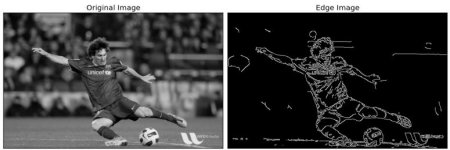
\includegraphics[width=0.7\textwidth]{./images/openCvCannyExample.jpg}
	\caption{Opencv example of canny detection, source \citep{opencv_library} docs}
	\label{am:cannyexample}
\end{figure}


\begin{figure}[h!]
	\centering
	\includegraphics[width=0.7\textwidth]{./images/openCvCannyGolfCourse.png}
	\caption{OpenCV canny edge detection on an image of a golf course}
	\label{am:CannyGolfCourse}
\end{figure}

\begin{figure}[h!]
	\centering
	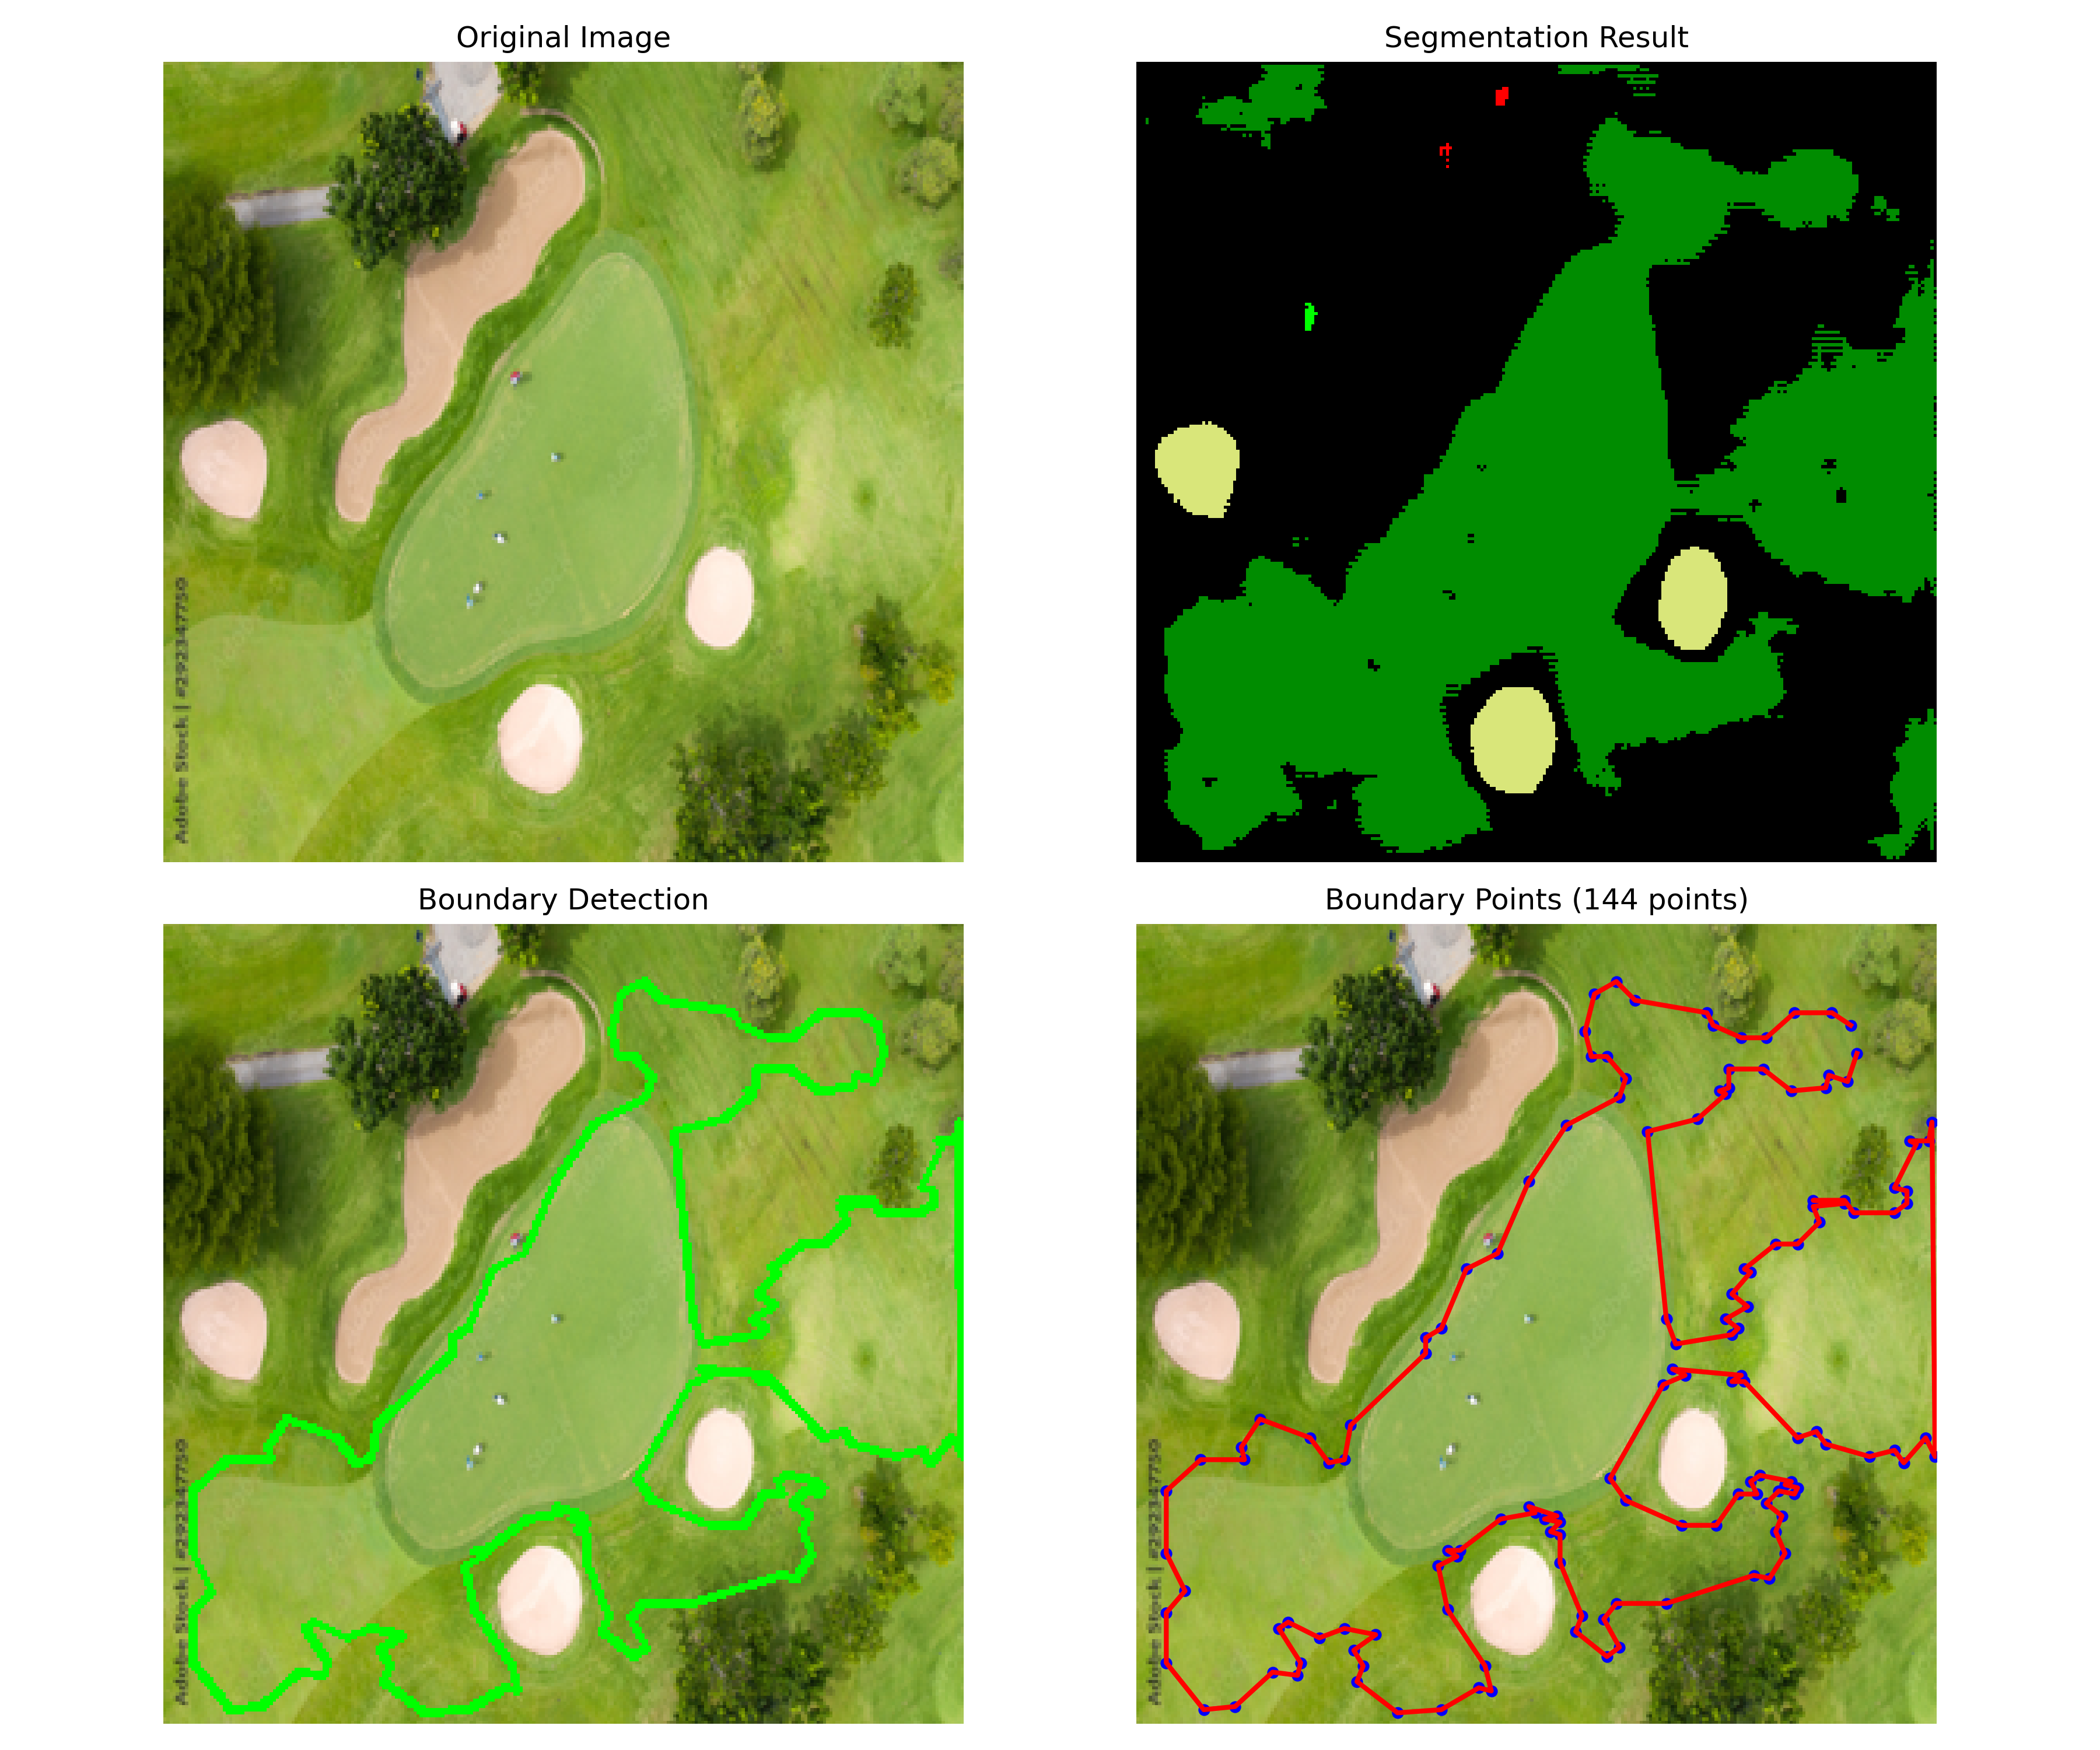
\includegraphics[width=0.7\textwidth]{./images/AdobeGolf_visualisation.png}
	\caption{An example ouput of pytorch model trained on the Danish Golf Course data set}
	\label{am:AGDanish}
\end{figure}

\begin{figure}[h!]
	\centering
	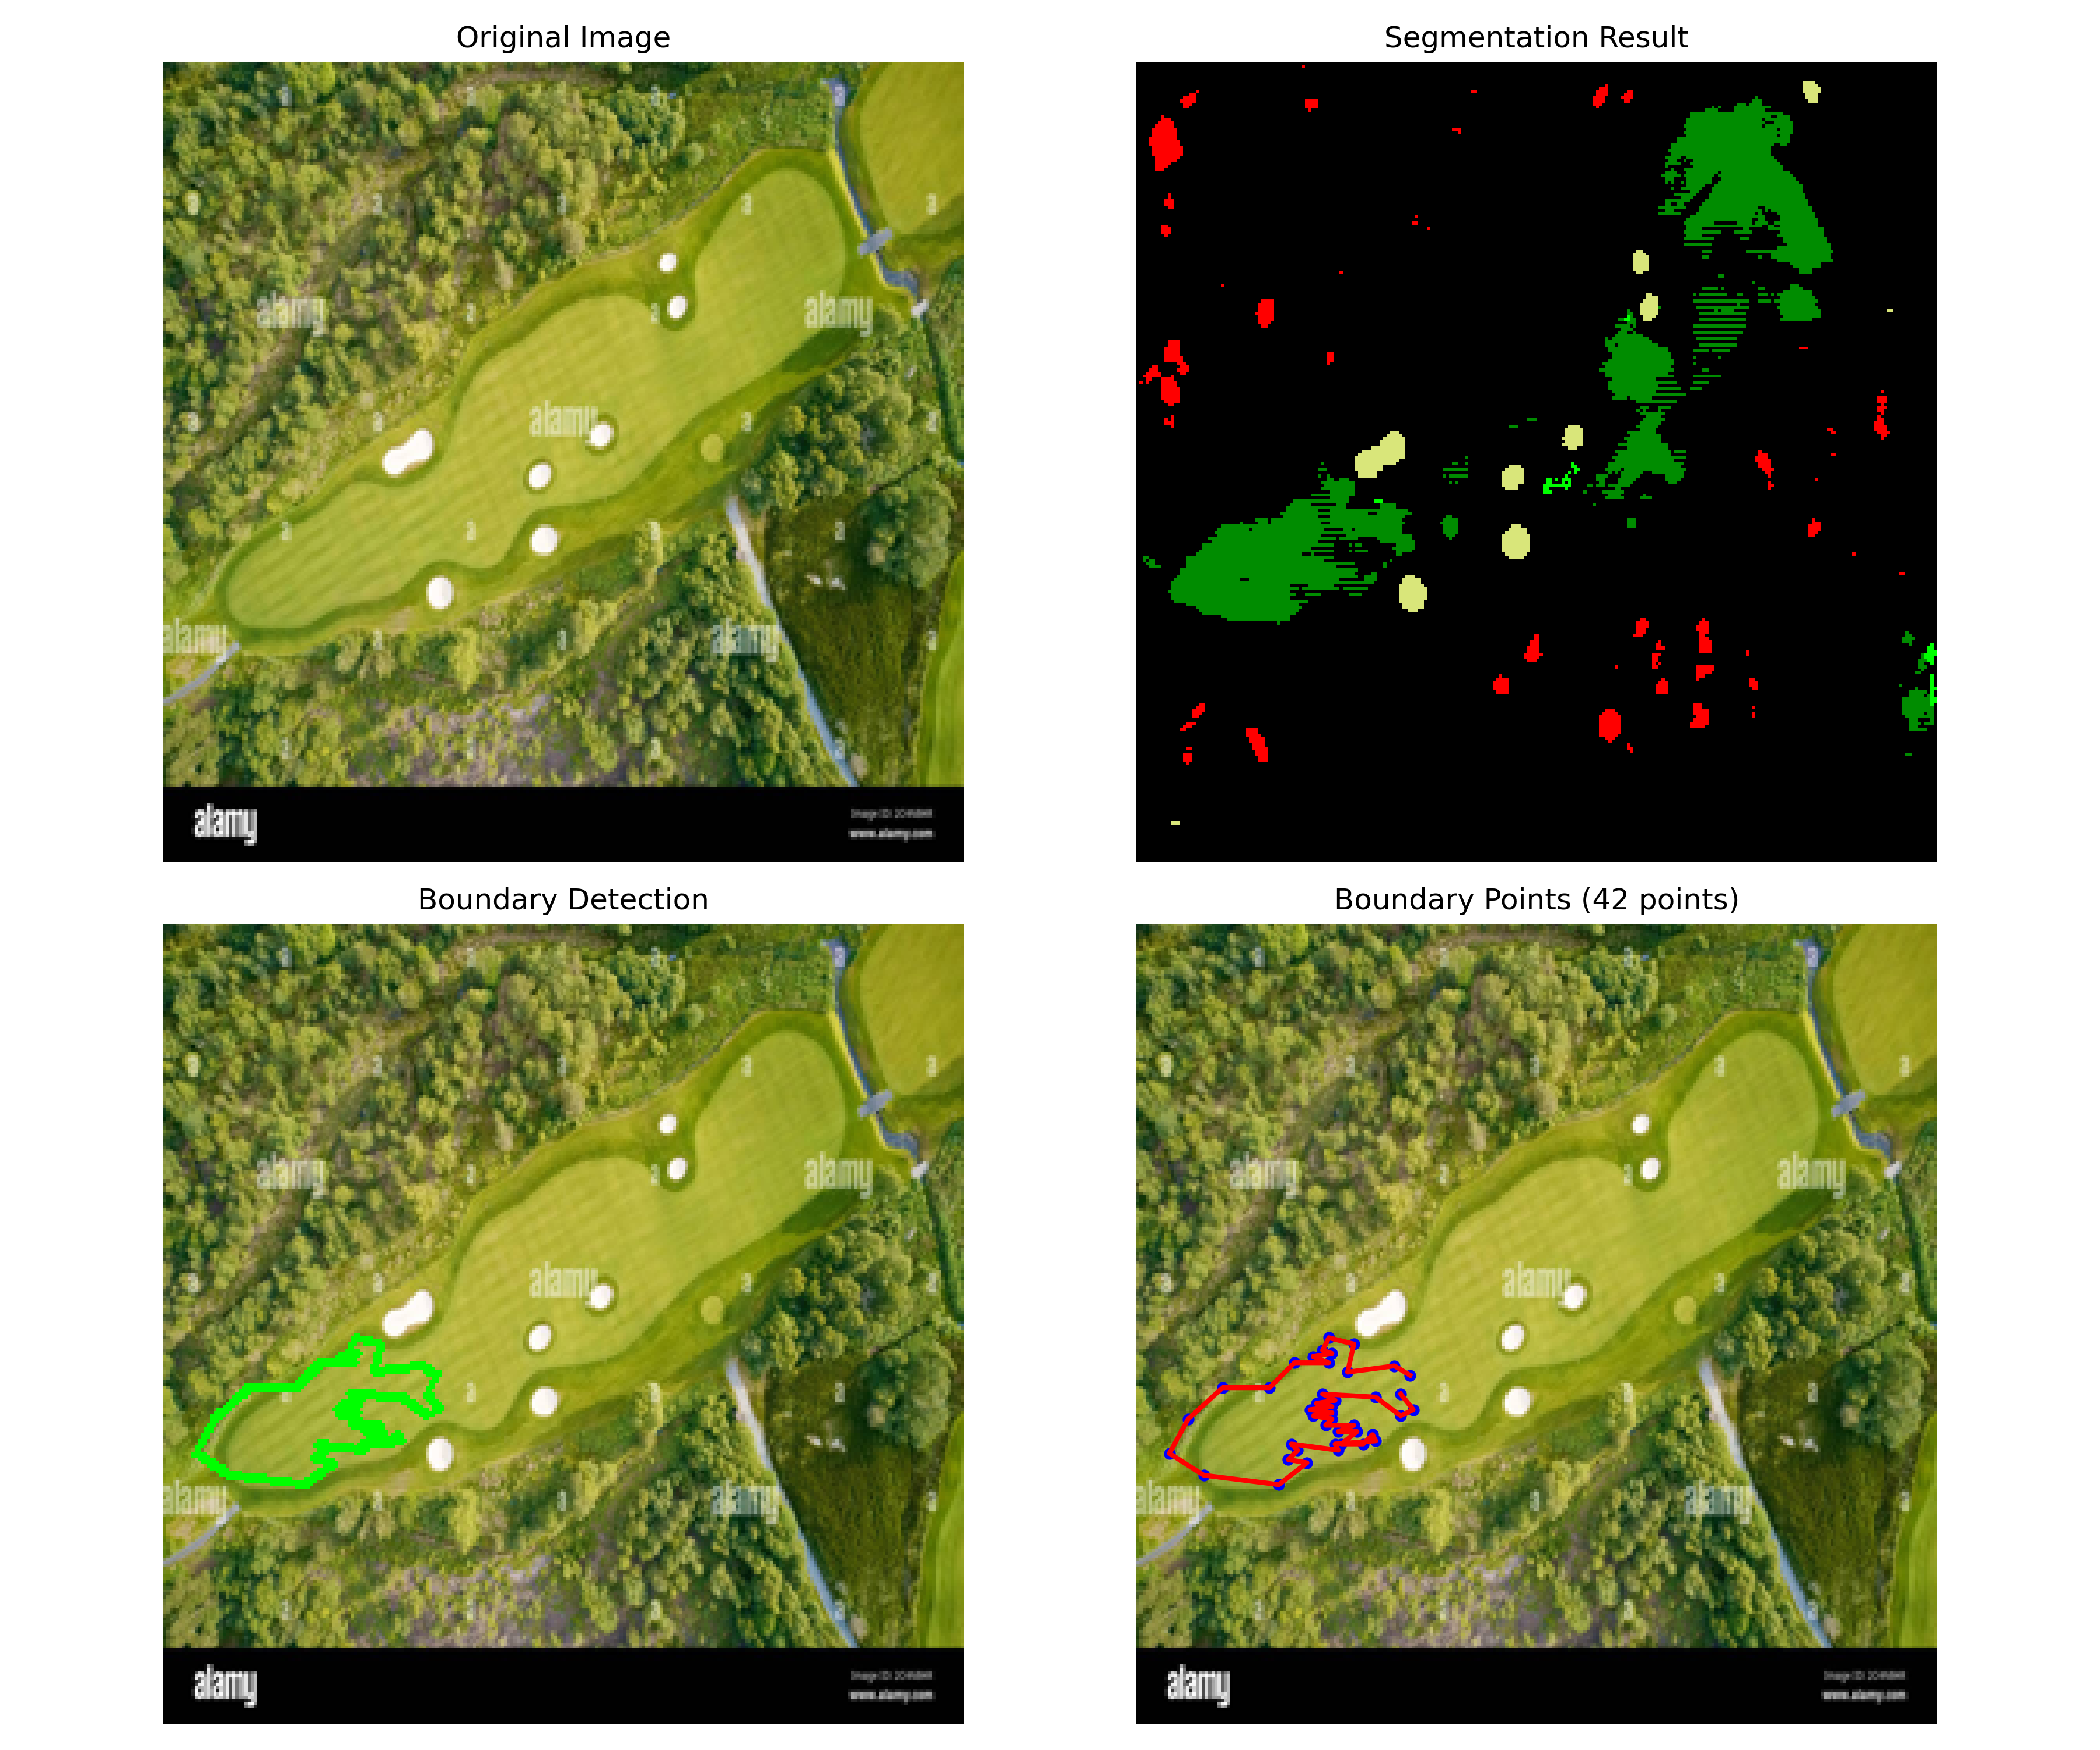
\includegraphics[width=0.7\textwidth]{./images/overheadGolfCourse_visualisation.png}
	\caption{An example ouput of pytorch model trained on the Danish Golf Course data set}
	\label{am:ohGCDanish}
\end{figure}

\section{Performance and Evaluation}
\subsection{Mapping}


\begin{figure}[h!]
	\centering
	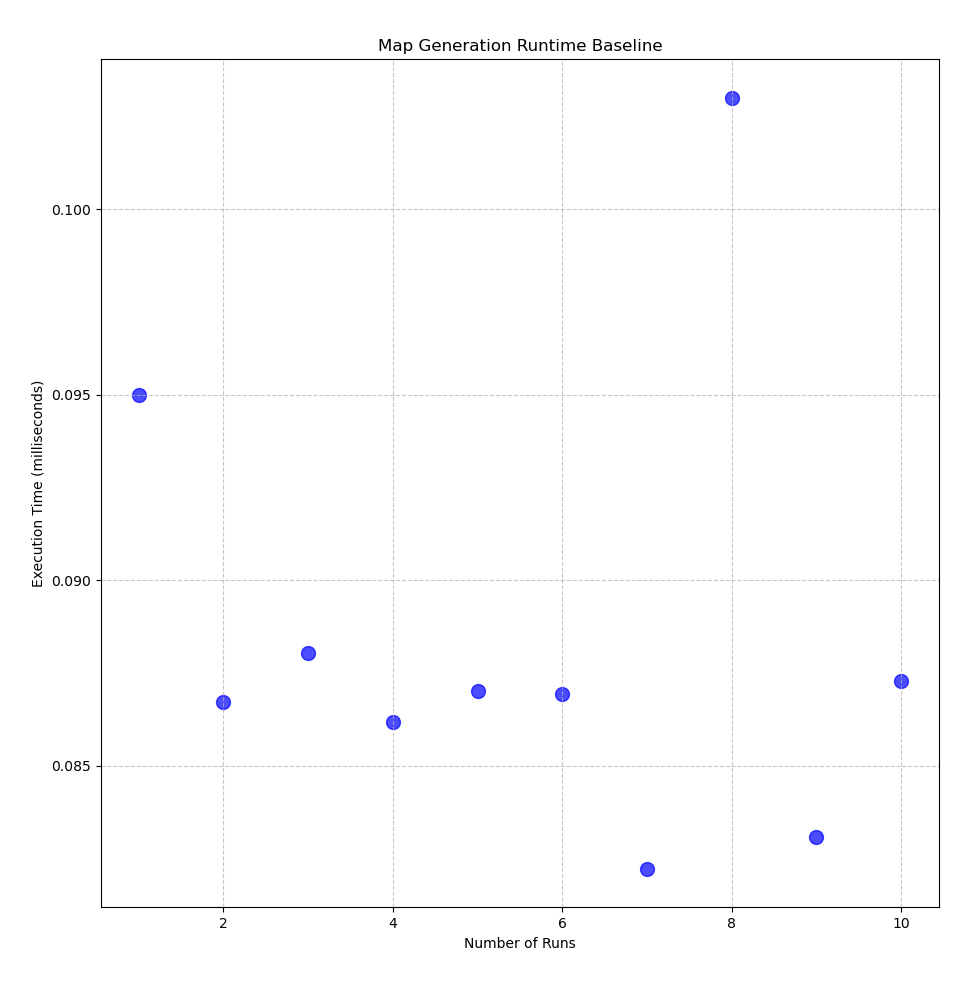
\includegraphics[width=0.5\textwidth]{./images/mapGenBaselineRT.png}
	\caption{Runtime of the map generation algorithm with 10 points, 400 range, 0 holes}
	\label{PE:mg:baselineRT}
\end{figure}


\begin{figure}[h!]
	\centering
	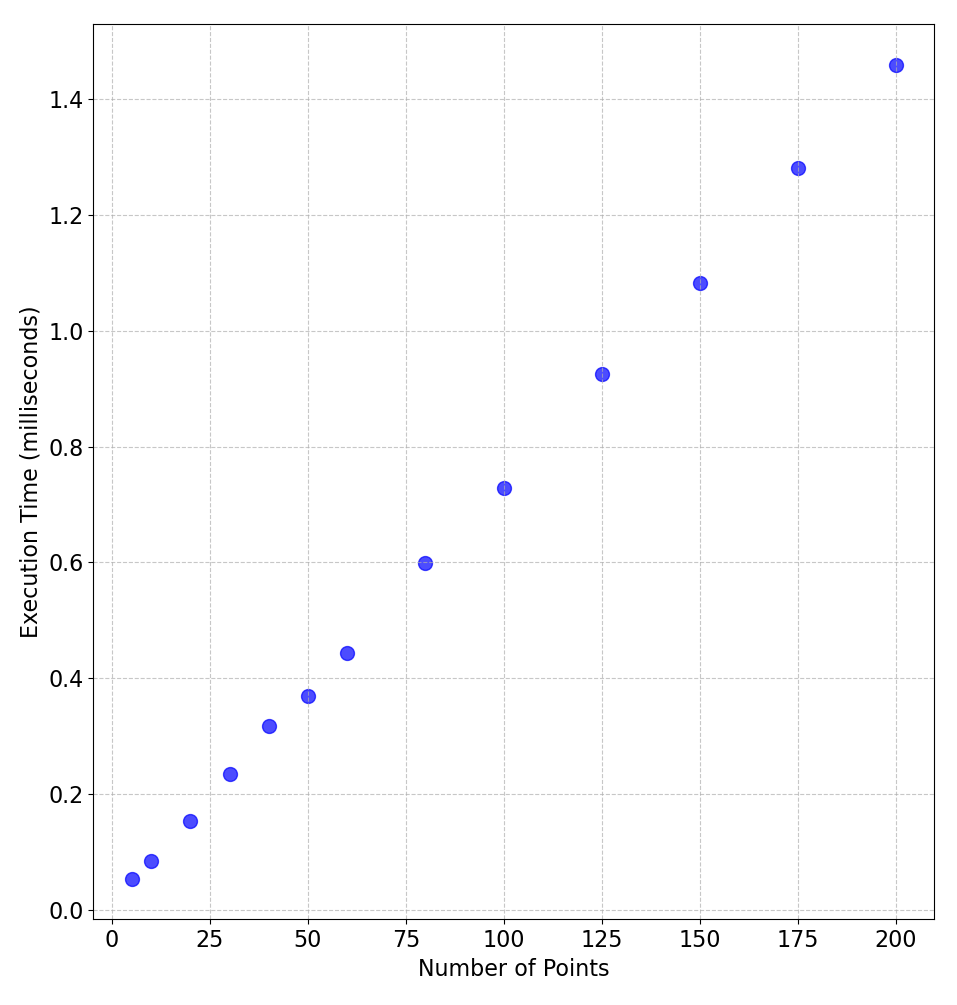
\includegraphics[width=0.5\textwidth]{./images/mapGenPointsRT.png}
	\caption{Runtime of the map generation algorithm with variable points, 400 range, 0 holes}
	\label{PE:mg:points}
\end{figure}


\begin{figure}[h!]
	\centering
	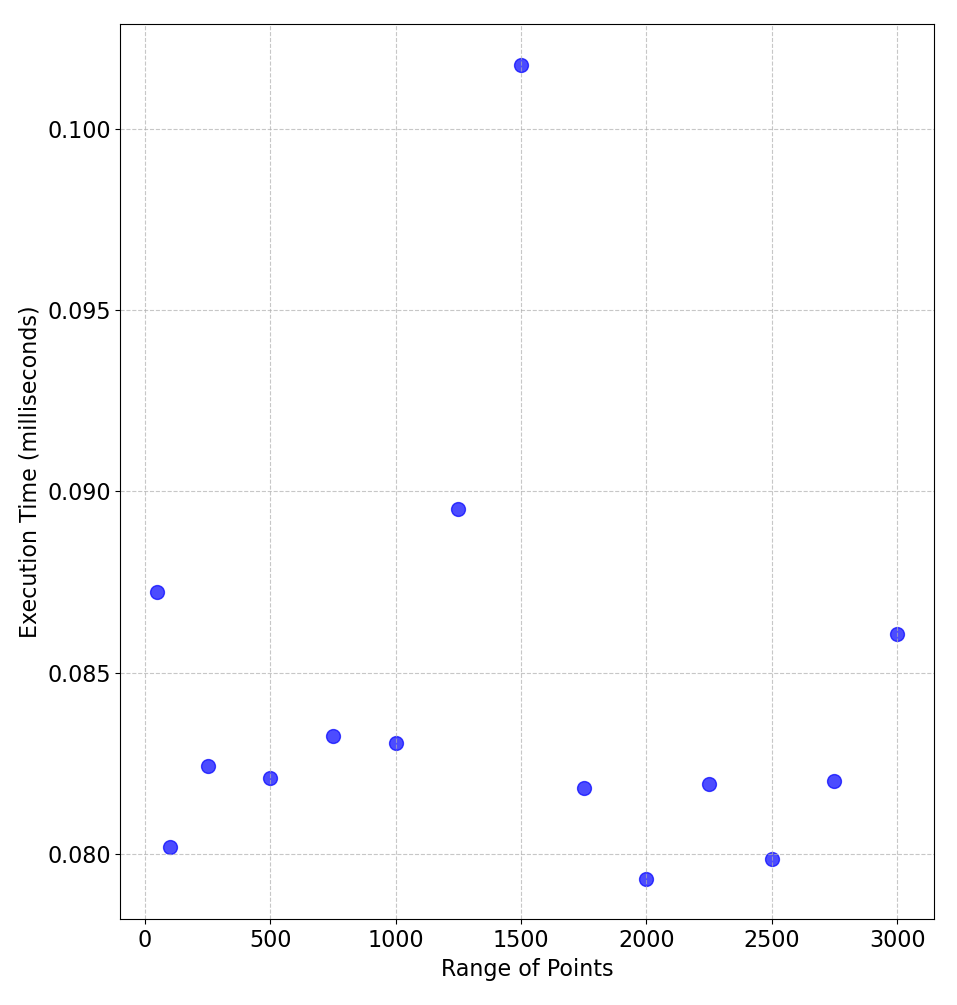
\includegraphics[width=0.5\textwidth]{./images/mapGenRangeRT.png}
	\caption{Runtime of the map generation algorithm with 10 points, variable range, 0 holes}
	\label{PE:mg:range}
\end{figure}

\begin{figure}[h!]
	\centering
	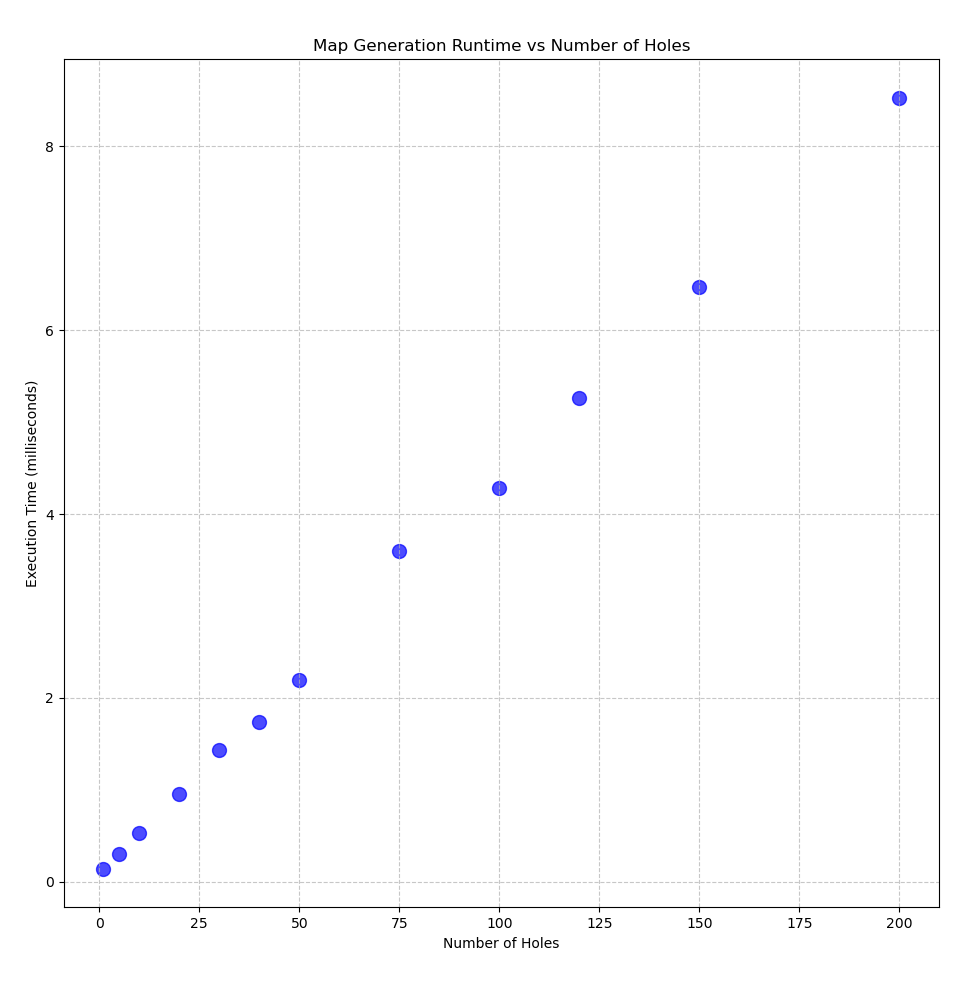
\includegraphics[width=0.5\textwidth]{./images/mapGenHolesRT.png}
	\caption{Runtime of the map generation algorithm with 10 points, 400 range, variable holes}
	\label{PE:mg:holes}
\end{figure}

\begin{figure}[h!]
	\centering
	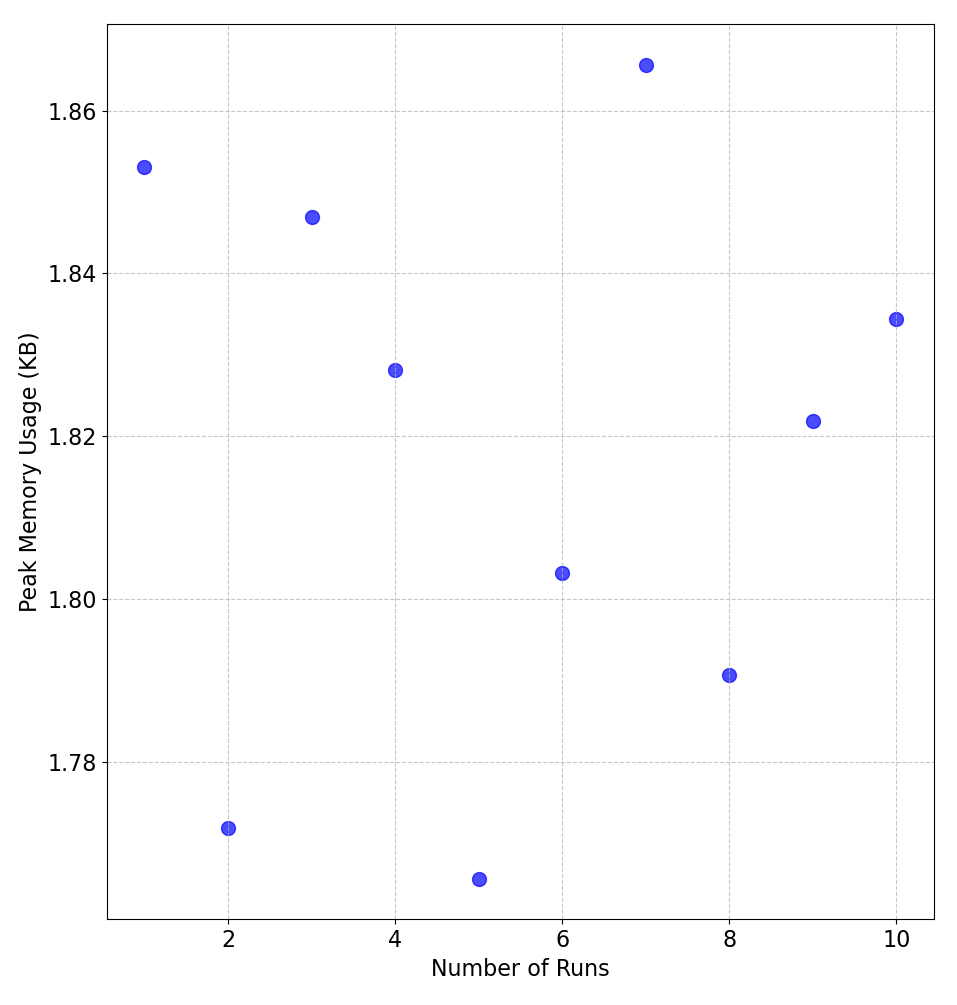
\includegraphics[width=0.5\textwidth]{./images/mapGenBaselineMem.png}
	\caption{Memory usage of map generation algorith with 10 points, 400 range, 0 holes}
	\label{PE:mg:memBaseline}
\end{figure}

\begin{figure}[h!]
	\centering
	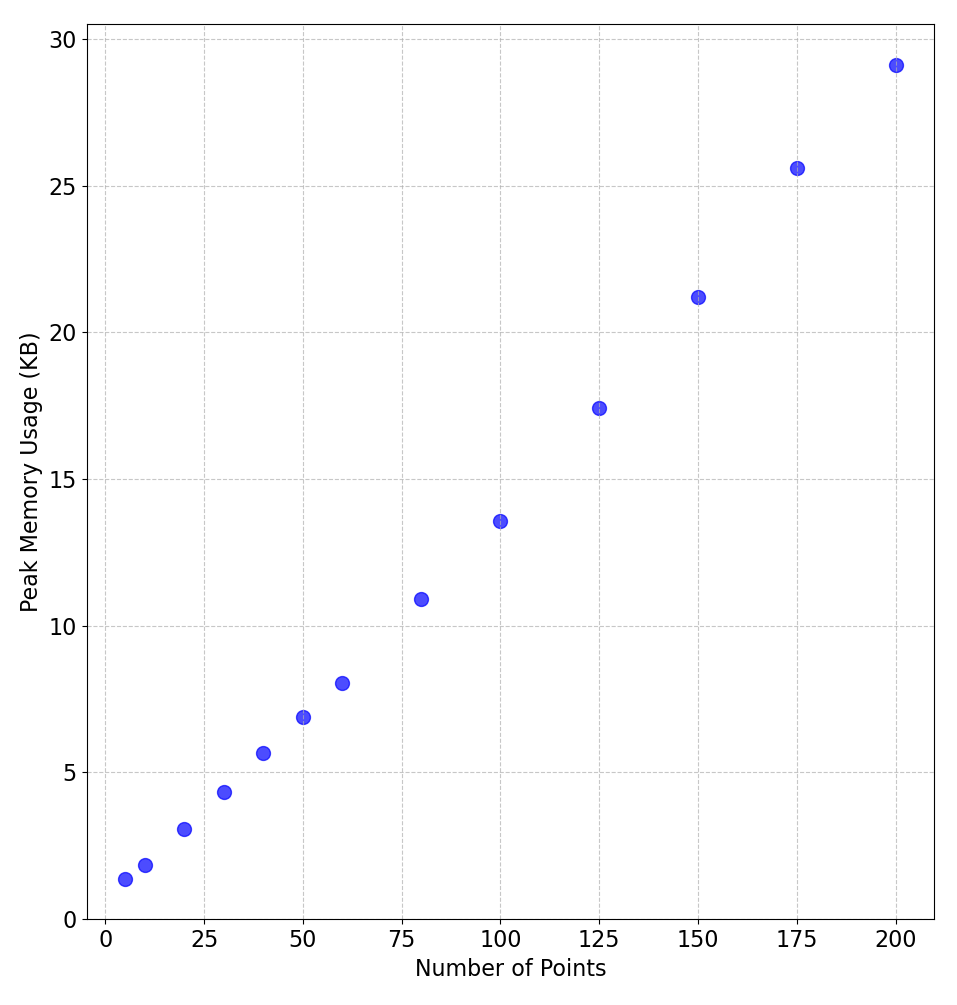
\includegraphics[width=0.5\textwidth]{./images/mapGenPointsMem.png}
	\caption{Memory usage of map generation algorith with variable points, 400 range, 0 holes}
    \label{PE:mg:memPoints}
\end{figure}

\begin{figure}[h!]
	\centering
	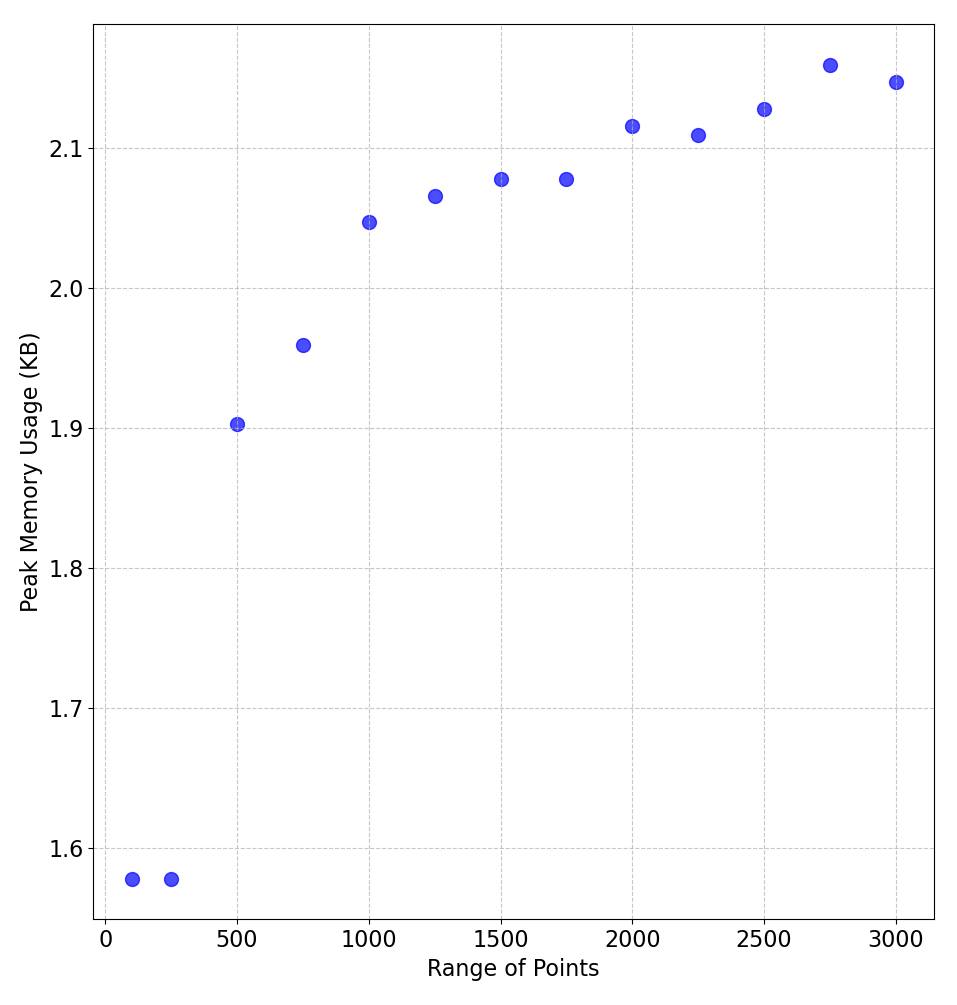
\includegraphics[width=0.5\textwidth]{./images/mapGenRangeMem.png}
	\caption{Memory usage of map generation algorith with 10 points, variable range, 0 holes}
	\label{PE:mg:memRange}
\end{figure}

\begin{figure}[h!]
	\centering
	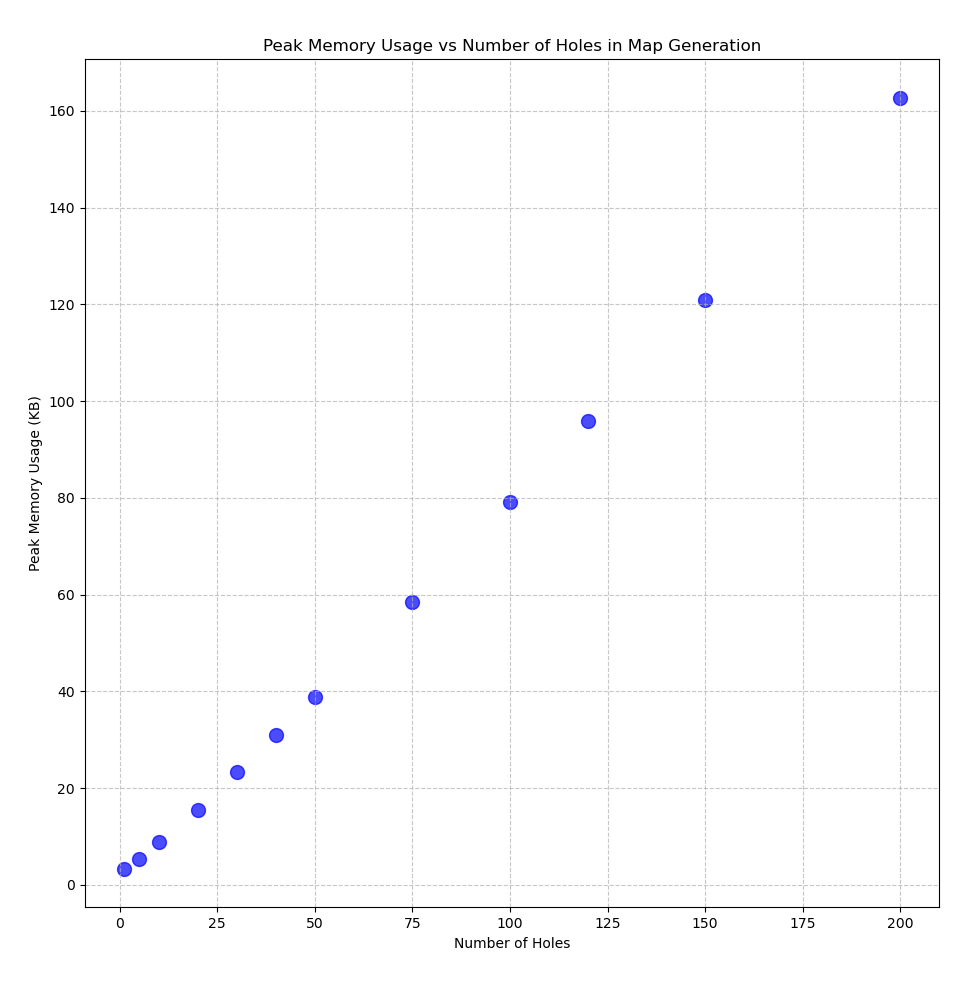
\includegraphics[width=0.5\textwidth]{./images/mapGenHolesMem.png}
	\caption{Memory usage of map generation algorith with 10 points, 400 range, variable holes}
	\label{PE:mg:memHoles}
\end{figure}


\begin{figure}[h!]
	\centering
	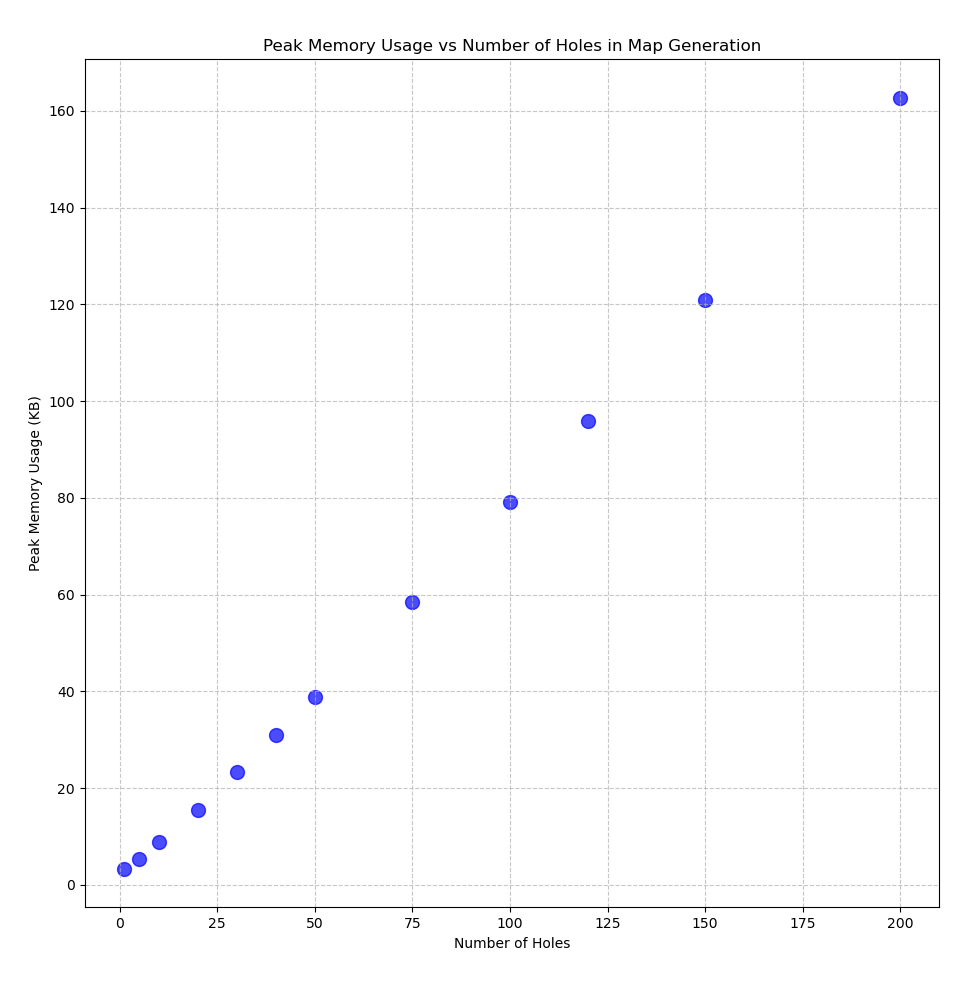
\includegraphics[width=0.5\textwidth]{./images/mapGenHolesMem.png}
	\caption{Runtime of path planning system with }
    \label{PE:p:setSize}
\end{figure}




\end{document}
